\chapter{16 Tales - Volume 4}

\begin{figure}[H]
    \centering
    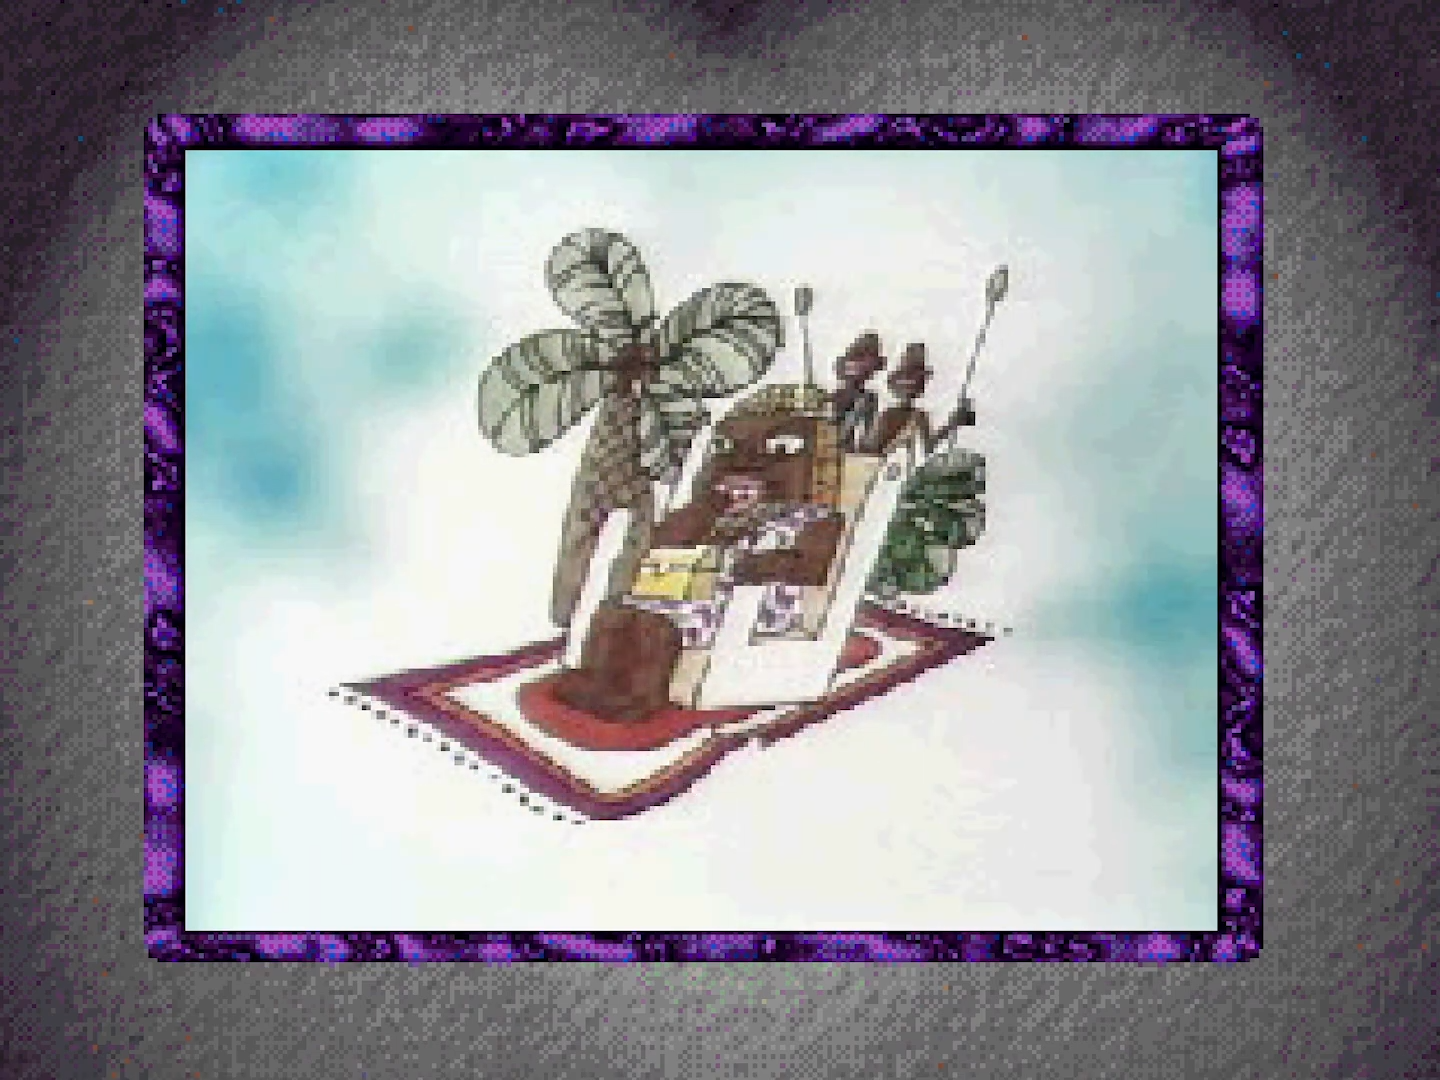
\includegraphics[width=\textwidth/2]{"./Games/16Tales/Images/16Tales4Screenshot.png"}
    \caption{16 Tales 4 Screenshot}
\end{figure}

The fourth of the four 16 Tales games published and released by The Lightspan Partnership for the PlayStation 1.

16 Tales - Volume 4 features four 15-minute video programs detailing the following African stories:

\begin{itemize}
    \item Anance and the Golden Box
    \item Brer Rabbit and the Tar Baby
    \item How Anance Got a Thin Waist \& Ananse's Visitor Turtle
    \item Wakaima and the Clay Man
\end{itemize}

\clearpage
\newpage

\section{Anance and the Golden Box}

\subsection{Audio Summary}

Anance and the Golden Box comes from West Africa where the Ashanti people live. It tells of a time when there were no stories to be told, and how Anance the spider man convinces Nyamey the sky god to share his golden box of stories with the world.

\subsection{Transcriptions}

Africa is a land of many countries, towns, villages and tribes, a land of varied customs, dressed in languages; therefore a land of many people.

Come with me along Africa's West Coast to Nigeria on the Gulf of Guinea where more pure negroid people live than anywhere else in the world.

Come to Ghana where the Ashanti live. Long ago, the Ashanti came to this land from somewhere farther north. No one really knows where. They cleared and planted the Earth and hunted the wild game of the forest. Among the Ashanti were fine artists and craftsmen, weavers, metalsmiths, wood carvers and drum makers. They had their poets, singers and storytellers. The storytellers passed on the legends of the migration of their ancestors, stories of their heroes, stories of how the world began and how certain customs came to be.

Today, life among the Ashanti has changed, as life everywhere is changing. The king of Ashanti lives in a modern house and works in an office much like our president. But the old traditions and customs are not forgotten. Even today, in the Ashanti villages, children gather at night to hear their favorite stories.

Most are about the spider. The Ashanti tribe is said to have created the tales of Quako Ananse, a cunning spider who appears as Spider the animal or Spider the man. He is, at the same time, the wisest and most stupid of all creatures, sometimes a hero and sometimes a smart alec whose schemes don't always work out. All tales are called anansium in honor of the spider Ananse. But wait, come with me and hear how such a strange thing came to be. Listen, hear the storytellers call.

"Come, come, come listen to the time when there were no stories on Earth to hear. Come listen, listen and learn."

Once, so they say, they say, a long, long time ago, ago, there were no stories on the earth to hear. All of the stories belong to Nyamey. Nyamey was the sky God. He kept the stories in a golden box on his royal throne.

Now Ananse, the Spider-Man, thought it would be nice to have some stories to tell, so he decided to visit the sky God, Nyamey. He spun a magic web and climbed up, up, up, up into the sky until he reached the home of the sky God. When Nyamey, the sky God, heard what Ananse wanted, he laughed.

He said to Ananse, 'If you want my stories, there is a price you must pay. You must bring me Osable, the leopard of the terrible teeth, and you must bring me Mboro, the Hornet who stings like fire, and last of all, you must bring me Mwatia, the fairy whom men never see.'

Ananse bowed and said to Nyamey, 'I shall gladly pay your price. I shall bring you Osable, the leopard of the terrible teeth, Mboro, the Hornet who stings like fire, and even Mwatia, the fairy whom men never see.'

Again the sky God laughed. He thought, 'How can Ananse pay my price? He is a weak old man and is so small, so small, so small.'

Ananse left the sky God and began his journey back to Earth to find the things that the sky God demanded. He climbed down, down, down, down his web. The next day, Ananse was walking along a jungle path and he came face to face with Osable, the leopard of the terrible teeth.

'Hello Ananse,' said the leopard. 'You are just in time to be my lunch.'

Ananse said, 'Hmm, as for that, what will happen will happen. But first, why don't we play the Binding game?'

Now the leopard, who liked to play games, asked, 'How do you play this game?'

'With vine ropes,' explained Ananse. 'I will tie you up foot to foot, then I will untie you and then it's your turn and you can tie me up.'

'Very well,' growled the leopard. He planned to eat Ananse as soon as it was his turn to tie him up.

So Ananse tied up the leopard foot to foot, to foot, to foot with the vine ropes. Then he said, 'Now, O Sable, you are ready to meet the sky God.'

Ananse found a tall tree and then he hung the leopard from a branch. The angry leopard watched as Ananse cut a banana leaf from a banana tree and filled the gourd with water. Ananse crept through the tall grass, very softly, very softly, very softly, until he came to the nest of Mboro, the Hornet who stings like fire.

Ananse held the banana leaf over his head like an umbrella. He poured some of the water from the gourd over his own head. He poured the rest over the Hornet's nest and cried, 'It's raining, it's raining, it's raining! Would you like to fly into my gourd so that the rain will not tatter your wings?'

'Thank you very much, oh thank you very much,' hummed the Hornets, and flew into the gourd.

Ananse quickly put the stopper in the mouth of the gourd. 'Noq Mboro, you are ready to meet the sky God,' said Ananse, as he hung the gourd full of hornets on the tree next to the leopard.

Next, Ananse carved a little wooden doll, holding a bowl. He carefully covered the doll from top to bottom with sticky tree gum. Then he filled the doll's bowl with pounded yams. He set the little doll at the foot of a flamboyant tree where fairies like to dance.

Ananse tied one end of a vine around the doll's head and, holding the other end in his hand, he hid behind a bush. In a little while, Mwatia, the fairy whom men never see, came dancing, dancing, dancing to the foot of the flamboyant tree. There she saw the doll holding the bowl of yams.

Mwatia said, 'little gum baby, I am hungry. May I eat some of your yams?'

Ananse pulled the vine from his hiding place so that the doll seemed to nod its head.

So the fairy took the bowl from the doll and she ate all of the yams.

'Thank you, little gum baby,' said the fairy. But the doll did not answer.

'Don't you answer when I thank you?' asked the angry fairy. Of course, the doll did not move.

'Little gum baby, I'll slap your face unless you answer me,' shouted the fairy. But the wooden doll remained silent.

So the fairy slapped the doll. Pow! Her hand stuck to the doll's sticky cheek.

'Let go of my hand or I'll slap you again!' Pow! She slapped the doll's face with her other hand. Now the fairy was stuck to the doll with both hands and she was furious. Then she pushed against the doll with her feet and they also stuck fast.

Now Ananse came out of his hiding place. 'You, Mwatia, are ready to meet the sky God,' and he carried her to the tree where the leopard and the hornets were waiting.

Then Ananse spun a web around the leopard and around the hornets and around the fairy. He spun and spun until he had them all in a bundle. Then he began to spin a web up to the sky. He pulled up his captives behind him and climbed and climbed and climbed his web to the home of the sky God, Nyamey.

When he arrived, he placed the bundle at the feet of the sky God. 'Nyamey, god the blue sky, here is the price for your stories,' said Ananse as he bowed.

Nyamey, the sky God, called together all the nobles of his court and said to them in a loud voice, 'Here see, here see, little Ananse, the Spider-Man, he has paid me the price I asked for my stories. From this day on,' proclaimed the happy sky God, 'my stories belong to Ananse, the Spider-Man, and shall be called spider stories.'

'Hooray, hooray, hooray,' shouted the assembled nobles.

Ananse, the Spider-Man, took the golden box of stories and climbed down, down, down his web back to the Earth to the people of his village. And when Ananse opened the box, all of the stories, including this one, scattered to all the four corners of the world.

Now we know why it is said that Ananse gave us all our stories. When Africans came to the new world as slaves or as free men, they brought along their Ananse tales. Sometimes the places and characters were changed, but the meanings of the stories remained the same. Today there are many stories about Ananse. They are told in Africa, the West Indies, in South and Central America, and of course, in the United States. Ananse the spider has several different names, and the stories may be called Ananse stories or stories of Aunt Nancy or Sister Nancy.

Go, read. Read and share the tales of Ananse.

\subsection{Credits}

Told by: Janet MacLachlan,
Producer: K. Hamamura Nelson,
Executive Producer and Director: Edmond R. Chavanette,
Story Editor: Winnie Pearl Palmer,
Illustrator: Bob Smith,
Titles and Set: Doug Stiles,
Lighting: Ron A. Vanicek,
Technical Director: Bill Bolle,
Audio: Larraine E. Wilson,
Video: Roger Knipp,
Videotape: Clarence Pemberton,
Camera: John C. Merritt, Martin Miller, Ron A. Vanicek,
KLCS Los Angeles Unified School District

\section{Brer Rabbit and the Tar Baby}

\subsection{Audio Summary}

The folktale, Br'er Rabbit and the Tar Baby, is associated with the southeastern United States.
It originally came to the Americas with the slaves from Africa.
Br'er appears helpless and frightened, but in this story he is brave and intelligent, and outwits Br'er Fox and Br'er Bear.

\subsection{Transcriptions}

Today's story is an old favourite. It's called 'Br'er Rabbit and the Tar Baby'. The tar baby is considered part of the traditional folklore of the United States, but the story originally came from Africa.

Black American slaves were first brought from Africa to the Southern United States. They brought with them the memories of Africa and the way they used to live. They brought the richness of the tales and the legends of their people. In African tales, the animal characters were the rabbit Wakiama, the Spider Ananse, and the Tortoise and the Hare.

Our friend Br'er Rabbit is very similar to the rabbit Wakiama. Br'er Rabbit, like Wakiama, appears to be frightened and helpless, but he's really very smart. He's a practical joker and almost always outsmarts the bigger and stronger animals. Because he was so quick-witted, Br'er Rabbit was a favorite story character among the black slaves. The stories of his cunning gave them hope that they too might someday be free.

The Br'er Rabbit stories were collected by Joel Chandler Harris. The storyteller who gave him these stories was Uncle Remus, a black American slave. So let's hear the story of the tar baby and you'll get the feeling of the people of Africa and the southern plantation in America, when you hear the storytellers call, "Come, come, come and listen to the tales of Uncle Remus. Come listen, listen and learn."

One day, Br'er Fox and Br'er Bear was sitting in the woods talking about Br'er Rabbit, and they agreed that he was getting much too bossy and was sticking his nose into everyone's business.

"Br'er Rabbit is getting much too biggity," said Brother Bear.

"Yeah, someday I'm gonna catch Br'er Rabbit, and pull out his mustaches," said Br'er Fox.

"Someday I'm gonna catch Br'er Rabbit, and knock his head clean off, blim, blam, blim, blam," said Br'er Bear.

Then Br'er Fox thought of an idea. Now he was gonna catch Br'er Rabbit and he started to work right away. He got some tar and made it into the shape of a tar baby, with arms, legs, a stomach and a head. To make the tar baby look real, he pulled some hair from Br'er Bear's back and stuck them into the tar baby's head. And he took Br'er Bear's yellow hat and his own blue coat and put them on the tar baby.

"Come on now Br'er Bear, help me carry this tar baby down to the big road where that rabbit sure to come by."

And they put the tar baby under a tree by the side of the road and they hid in the bushes and waited for Br'er Rabbit to come by.

Well, it wasn't long before Br'er Rabbit came hopping down the road just whistling. Suddenly, he spotted the tar baby.

"How there!" said Br'er Rabbit. The tar baby didn't say anything. Br'er Fox and Br'er Bear watched from the bushes.

Br'er Rabbit waited for an answer. Then he said louder. "What's the matter with you? I said how do you do? Is you deaf? Now if you is, I can holla louder." The tar baby said nothing.

Then Br'er Rabbit yelled real loud, "Where is your politeness? Ain't you gonna say 'how do you do' like respectable folks say when they meet up on the road?"

The tar baby said nothing while Br'er Fox and Br'er Bear hid in the bushes.

Br'er Rabbit got real mad. "If you don't say 'howdy do' by the time I count three, I'm going to blip you in the nose." Br'er Rabbit counted. "One, two, three."

But still the tar baby said nothing, so he drew back his right fist and pow. Hit the tar baby right in the nose. But his fist stuck in the tar and he couldn't pull it loose.

Br'er Rabbit got madder. "Let go of my fist, y'all," and he drew back his other fist and again he hit the tar baby in the nose. This fist stuck in the tar too and he couldn't get either hand loose.

The tar baby said nothing. Br'er Fox and Br'er Bear started to laugh in the bushes.

"You don't let go my fists," yelled Br'er Rabbit, "I'm going to kick your teeth right out your mouth."

Well Br'er Rabbit pulled back one foot and hit the tar baby, and his foot stuck. So he kicked with his other foot and kicked the tar baby again. Now both feet were stuck in the tar.

"If you don't let go of my foot, if you don't let go of my foot," screamed Br'er Rabbit to the tar baby, "I'm gonna butt you with my head till you ain't got a breathe left in your body."

Br'er Rabbit butted the tar baby with his head, but his head got stuck in the tar. Now he was completely stuck, head, feet and fists, and the harder he tried to get unstuck, the more stuck he got.

Now Br'er Fox and Br'er Bear came out of the bushes feeling very good and they danced around Br'er Rabbit.

"We sure catched you this time, Br'er Rabbit," said Br'er Bear.

"Yeah, you better say your prayers, Br'er Rabbit. Cus this time is the very last day of your life."

Now Br'er Rabbit was starting to tremble. He was in big trouble, but he set his mind to work to figure out how he could get out of this mess. Br'er Fox and Br'er Bear was so happy that now they were trying to figure out what to do with Br'er Rabbit.

Br'er Bear wanted to knock his head clean off, but Br'er Fox wanted to make him suffer.

"Br'er rabbit," he said. "You've been sticking your head into my business for years, but now I got you and I'm gonna fix up a big fire and one that's good and hot. I'm going to drop you in and roast you."

Br'er Rabbit wasn't scared anymore. He had an idea how he could get loose, but he talked like he was very scared.

"I don't care what you do with me," he said. "Just don't fling me over that these bushes into that there Briar Patch. Just, just as hot as you please, you can roast me. But don't fling me into that dare Briar Patch."

Br'er Bear got to thinking. If they roasted Br'er Rabbit, that would mean that they'd have to go gather wood for the fire and that meant work.

Br'er Fox said, "well then, Br'er Rabbit, I'm going to hang you."

"Well, hang me just as high as you please," said Br'er Rabbit to Br'er Fox. "But please, don't fling me in that there Briar Patch."

Br'er Bear started thinking again. Now to hang Br'er Rabbit, they'd have to get a long rope. So Br'er Fox decided to drown Br'er Rabbit.

"Drown me just as deep as you please," said Br'er Rabbit. "But just please, please, don't fling me in that there Briar Patch."

"It's gonna be a whole lot of trouble to drown Br'er Rabbit," said Br'er Bear. "First we'd have to carry him all the way down to the river."

"That's so," said Br'er Fox. "Well Br'er Rabbit, I expect the best way here's to skin you. Come on, Br'er Bear, let's get started."

"Skin me, skin me," said Br'er Rabbit. "Pull out my ears and snatch off my legs. You can chop off my tail, but please, please, Br'er Fox and Br'er Bear, don't fling me in that dare Briar Patch."

Br'er Bear started to grumble and he told Br'er Fox that Br'er Rabbit wasn't scared of being skinned, so it wouldn't be much fun to skin him.

"He sure is scared of that Briar Patch," said Br'er Fox.

"That's just where he gonna go. This is the end of you, Br'er Rabbit."

Br'er Fox pulled Br'er Rabbit from the tar baby and threw him into the middle of the Briar Patch. There was a lot of noise and activity when Br'er Rabbit landed in the Briar Patch. He was yelling and carrying on, making a real big ruckus. After quite a time, the noise started to quiet down, with only an occasional tired yell.

Br'er Fox and Br'er Bear had been listening, smiling, and they shook hands and slapped each other on the back.

"Br'er Rabbit ain't gonna be too sassy no more," said Br'er Fox.

"Br'er Rabbit ain't gonna be too bossy no more," said Br'er Bear.

"Br'er Rabbit ain't going to do nothing no more," said Br'er Fox, and Br'er Bear. "This is the end of the rabbit. Br'er Rabbit is dead."

Just then, Br'er Fox and Br'er Bear heard a lot of noise among the leaves at the other end of the Briar Patch. And who do they see come scrambling out of the bushes: none other than Br'er Rabbit. He was singing and whistling and combing the last bit of tar out of his mustache with a piece of Briar brush.

"Howdy Br'er Fox and Br'er Bear," he yelled. "I've told you and told you not to fling me in that dare Briar Patch. That's the place in all this world I love the very best. That Briar Patch is the place where I was born."

And with that, Br'er Rabbit hopped off down the road, laughing so hard he couldn't laugh anymore.

Now that's a smart rabbit. There are many more stories of Br'er Rabbit, Br'er Bear, Br'er Fox and all our friends, all collected by Joel Chandler Harris. So go, read, and share the tales of Uncle Remus. Go read: read and learn.

\subsection{Credits}

Told by: Chuck Douglas,
Producer: K. Hamamura Nelson,
Executive Producer and Director: Edmond R. Chavanette,
Story Editor: Winnie Pearl Palmer,
Illustrator: Camille Higgins,
Titles and Set: Doug Stiles,
Lighting: Ron A. Vanicek,
Technical Director: Bill Bolle,
Audio: Larraine E. Wilson,
Video: Roger Knipp,
Videotape: Clarence Pemberton,
Camera: John C. Merritt, Martin Miller, Ron A. Vanicek,
KLCS Los Angeles Unified School District

\section{How Anance Got a Thin Waist \& Ananse's Visitor Turtle}

\subsection{Audio Summary}

In our first story, How Anance Got a Thin Waist, we will learn why spiders have a thin middle, and in the second story, Ananse's Visitor Turtle, we'll see what happens when Ananse tries to get a free meal from the turtle.

\subsection{Transcriptions}

Our stories today come from West Africa, from Ghana, where the Ashanti people lived. Long ago, the Ashanti came to Ghana from somewhere farther north. They cleared and planted the land and hunted wild game of the forest. Among the earliest Ashanti were fine craftsmen, wood carvers and weavers.

The Ashanti of the past and the village people of today build their dome-shaped houses in a circle, using slender poles covered with woven grass reeds. Boys and girls help thatch the little houses with sheets of grass cut in short lengths.

And at night, when the moon is high in the sky and all a day's work is done, the men, women and children of all ages leave their round houses and go to an open space in the middle of the village. There they gather around a cozy fire and call for the storyteller: the one who tells the stories the best.

West Africa is rich in the number of different kinds of stories it's created. The folk tales of the Ashanti tribe are particularly noted for their humor, and it was the Ashanti who created the stories of Kwaku Ananse, the cunning spider. Ananse is one of the favorite West African characters. Sometimes he's a spider, and other times he appears as a man. He's at the same time both very wise and very foolish. Ananse loves to eat but he hates to work, and this often gets him into trouble, and he usually has to use his cleverness to get himself out of it.

In our first story, we'll learn why spiders have a thin, thin middle, and in the second story, we'll see what happens when Ananse tries to get a free meal from the turtle.

So imagine yourself in West Africa on the Gulf of Guinea,. The night is high and the moon is high in the sky. It's a time for storytelling. So gather around and hear: heard the storytellers call.

Come, come, come listen to the time when the spider was fat and had no thin. Come, listen to the time when the turtle outsmarted Ananse. Come listen, listen, listen and learn...

Early one morning, Ananse was walking through the forest when he noticed a very pleasant smell. He wrinkled his nose and sniffed the wind first. First this way, then that.

"Goodness me, it is food," he'd almost forgotten. Today was the Festival of the Harvest, and every village in the forest was preparing a feast. People were cooking yams and cassava and chicken with peanut-flavored sauce, and there would be fish and peppers and rice boiling in great pots.

Ananse jumped for joy and smacked his lips. His eyes sparkled and he smiled brightly as he thought of the good-tasting food. Now Ananse had not done any work to deserve such a feast, so no one had invited him to come and eat. All he did was play in the sun and sleep. Ananse was right in the middle of a path between two villages, and each village was having a feast.

"How lucky for me," thought Ananse. But he didn't know which feast to go to, so he sat down to think about it. He thought for a long time. Finally, he decided, "I shall go to both of them."

Ananse was so pleased with himself that he did a little dance. Now how could he know when the food was ready? He sat down to think some more. When he thought of a plan, he did another dance because he was so brilliant.

With his plan in mind, Ananse did two things. First, he called his eldest son Ntikuma. He took a long rope and tied one end around his middle and gave the other end to his son.

"Take this rope to the villages on the east and when the food is ready, give the rope a hard pull and then I'll know that it's time to come and eat," he said to Ntikuma.

Then Ananse called his youngest son Kwaku, and took another long rope, tied it around his middle just below the first one.

"Kwaku," he said, "now you take this rope to the village on the west, and when the food is cooked, pull very, very hard and then I'll come and eat my fill."

Well you can imagine what happened. The people in both villages had dinner at the same time. Of course, both of Ananse's sons pulled on the ropes at the same time. The ropes got tighter and tighter, and poor greedy Ananse was caught right in the middle. He could neither go east or west. Ntikuma and Kwaku couldn't understand why their father didn't come and both pulled harder and harder. The rope squeezed tighter and tighter and tighter, and his middle got thinner and thinner and thinner. Ntikuma and Kwaku waited until all the food was eaten, then they came to look for their father. When they found him, he looked very different. His waistline was thinner; thinner than a needle. Ananse never grew fat again. From that time on, he would have a big body and a tiny waist in between.

Many months later, when it was almost time for the sun to sink in its resting place, Turtle, tired and dusty from hours of wandering, came to Ananse's house in the middle of a clearing in the woods. Turtle was hungry and the smell of freshly cooked fish and yams drew him to Ananse's door.

Turtle knocked on the door. Ananse jerked open the door, and since it was the custom in his country to show hospitality to travelers, he smiled unhappily and invited Turtle to come in and share his dinner.

As Turtle reached out his paw for some food, Ananse stopped him. In a shocked voice, he said, "Turtle, in my country, it's bad manners to come to the table without washing. Please go to the stream and wash your dusty paws."

Turtle obediently waddled down the hill and waded in the water. He washed his paws, he even washed his face. By the time he got back to Ananse's house, half the dinner was gone and Ananse was eating very fast.

Turtle stretched out a paw to help himself to food, but again Ananse stopped him.

"Turtle," he said, "your paws are still dusty. Please go and wash them again."

"But it's dust from the trail," Turtle tried to explain, but he knew he shouldn't argue if he wanted to have any dinner.

So Turtle washed his paws in the stream again. On his way back to Ananse's house, Turtle walked in the grass by the trail, and he hurried because he was very hungry. But by the time the poor Turtle returned, Ananse had eaten all of the dinner and said, "That was a good dinner."

"Well thank you for your wonderful hospitality, Ananse. Some day, you must visit me," said the angry Turtle as he left to go home.

Some months later, Ananse visited the Turtle. After creepy-crawling all day through tall grass stems, he found Turtle snoozing by the river.

"Well, well, well," exclaimed the Turtle. "So you've come to share my dinner. Well, make yourself comfortable, Ananse, while I go below and prepare the food."

He dived into the river with a splash. Ananse was very hungry so he paced the shoreline waiting for Turtle to reappear. At last, Turtle's head popped above the water.

"Dinner is ready," he called to Ananse. "Come on down."

Ananse dived headfirst into the water, sank a few inches and then he floated to the surface. His spindly legs and tiny body prevented him from sinking. He flipped and flapped his puny arms and tried shallow dives and belly flops, but couldn't reach the bottom of the river, so the cunning spider schemed. He filled the pockets of his jacket with small round pebbles to make him heavier so he would sink to the bottom of the river. Again he dived into the water, but this time he went down, down, down and landed with a bump right at the dinner table. There before him was spread the most delicious meal he'd ever seen. There were oysters and clams and mussels and sliced eel and crabs. As a centerpiece, sprays of watercress rested against large pink shrimp.

Ananse's eyes widened with pleasure at the sight of such a feast. Turtle, already seated at the table, swallowed a piece of eel and looked at Ananse and said, "Ananse, look, I must remind you that in my country it is bad manners to wear a jacket to the table, so um, could you please take it off?"

So very slowly, Ananse removed his jacket, and very slowly, Ananse left the table. Without the weight of the pebbles to hold him down, he floated up, up, up, straight up to the top of the water.

Today, life among the Ashanti is as changing as life everywhere is changing. Life in the cities of West Africa is like city life anywhere. But the stories and the legends of long ago are still told and enjoyed. Today there are hundreds of stories about Ananse, stories like "How The World Got Wisdom", "How Spider Helped The Fishermen", and "How The Spider Got a Bald Head".

Ananse stories are told in Africa, in the West Indies, and in South and Central America. Of course, in the United States, you may hear them called the Ananse stories or stories of Aunt Nancy or Sister Nancy, but they're all stories about an adventurous spider.

So go, read: read and share the tales of Ananse.

\subsection{Credits}

Told by: Chuck Douglas,
Producer: K. Hamamura Nelson,
Executive Producer and Director: Edmond R. Chavanette,
Story Editor: Winnie Pearl Palmer,
Illustrator: Emerson Terry,
Titles and Set: Doug Stiles,
Lighting: Ron A. Vanicek,
Technical Director: Bill Bolle,
Audio: Larraine E. Wilson,
Video: Roger Knipp,
Videotape: Clarence Pemberton,
Camera: John C. Merritt, Martin Miller, Ron A. Vanicek,
KLCS Los Angeles Unified School District

\section{Wakaima and the Clay Man}

\subsection{Audio Summary}

Wakaima and the Clay Man tells the tale of how Wakaima, the lazy rabbit, tries to cheat his friend Wanjovu, the hardworking elephant, out of his crop, and how the sticky thief makes his escape.

\subsection{Transcriptions}

[Jambo watoto, karibu]. These are Swahili words of greeting, meaning "hello children, welcome". This is the language heard most in East Africa, a land of many races and ways of life. The people who live in the flatlands tend herds of animals. The people who live along the mountain slopes are farmers. But in the cities along the east coast, there are merchants and life is similar to city life anywhere in the world.

In the city and in the country, the tales and fables that were handed down years ago, before anyone could read or write, are still told. They are told in the evenings after sunset. The Swahili say, "[Akili apita mali]," which means "wisdom is better than wealth". And where better to find wisdom than in folk tales that have their origins in peoples from many places.

Stories of East Africa traveled from tribe to tribe long before there was a written language. Perhaps they were spread by traders or by a traveling storyteller. Listen, hear the storyteller's call. Listen, hear his call: come, come, come listen to the time when the rabbit and elephant were the best of friends. Come, listen, come listen and learn.

A long, long time ago, a rabbit lived in Africa by the name of Wakayima. Now, he was very, very lazy. His best friend was a big elephant whose name was Wanjovu. They both lived together on a farm. Wanjovu the elephant worked very, very hard, and Wakayima the rabbit was very lazy and did not work at all.

Now, Wanjovu got tired of living with a lazy rabbit, so one day he said, "I've got a great idea. Let's each have our own farm and we can share what we grow."

Wakayima agreed.

They each selected a piece of land. Wanjovu worked his soil and planted seed, but instead of working on his farm, lazy Wakayima ran off into the jungle and spent the day eating wild fruit and sleeping under the trees. When evening came, Wakayima rubbed dirt over his paws and face and stumbled into the house, groaning, rubbing his back and saying, "Oh, how hard I've worked. Oh, how tired I am."

Wanjovu was a good gardener and a hard worker. He planted corn, potatoes, peas and many other vegetables. When evening came, he was really tired, but he never complained.

One night, Wakayima crawled into the house with a stick or two for the fire; his paws and face covered with dirt.

"How tired I am. The work has been so hard today. I have worked all day without stopping."

Wanjovu believed him and prepared dinner for both of them, while Wakayima washed his paws and face before eating.

Now, one evening as they sat down to the dinner that Wanjovu had cooked, the elephant said, "Wakayima, you work much too hard on your farm."

The lazy Wakayima shook his head, then he said, "We can never work too hard. We must have plenty of food to store away before the rains come."

After many weeks passed, the crops were ready. The time had come to gather in the harvest. One evening, Wanjovu came home with a large basket filled with beautiful big ears of corn and fine white potatoes. He cooked them very carefully, and he and Wakayima sat down to eat.

"Mmm, how good the corn is, how sweet," said Wakayima. "I have never eaten finer potatoes."

The next evening, Wakayima came in with a basket full of corn and potatoes and said, "These are probably not as good as yours, but we will try them."

Wanjovu thought they looked very much like the corn and potatoes from his own garden, but he said nothing, knowing he would have to cook them and they would eat them for dinner.

The next morning when Wanjovu went to his farm, he saw that someone had stolen some of his corn and potatoes. That evening he told Wakayima, "Someone got into my farm last night and stole some of my vegetables."

Wakayima pretended to be very surprised. "Some thief got into my farm too," he said. "What are we going to do about it?"

Now we all know that Wakayima had stolen the vegetables from Wanjovu because he had no vegetables in his own garden.

"We must do something to keep the thief away," Wanjovu answered. "I will think of something and come up with a plan." But he did not tell his plan to Wakayima.

The next day, Wanjovu went to the river and got some clay. He worked all day and made a clay man with his arms outstretched. Carefully, he carried the clay man to his farm and set it down between the corn and potatoes. Later, when the moon rose, there stood the clay man, and there was his dark shadow, black in the white moonlight.

Now when Wanjovu had been asleep for many hours, Wakayima sneaked into Wanjovu's potato patch. Suddenly, Wakayima saw a giant figure in the moonlight and he was frightened. Could it be Wanjovu waiting to punish him for stealing the corn and potatoes? He didn't dare move.

The clay man didn't move. Finally, Wakayima gathered his courage to speak. "Hello, Wanjovu," he said. "What are you doing here at this time of the night?"

The clay man did not answer.

Wakayima began to lose his temper. "You are a thief who has come to steal Wanjovu's corn. Answer me or I will tell him."

The clay man did not answer.

Wakayima came nearer. He was puzzled. "Who are you and why don't you answer?" He demanded.

The clay man did not answer.

Wakayima cautiously walked around the clay man, who looked very, very large in the moonlight.

"If you don't answer me right now, I will hit you," shouted Wakayima.

The clay man still did not answer.

Wakayima hit the clay man hard with his paw and it stuck in the soft clay.

"Let me go or I'll hit you with my other paw," he screamed. The clay man did not let go.

Wakayima with his other paw punched the clay man in the stomach as hard as he could. This paw also stuck in the soft clay.

"If you don't let me go," shouted Wakayima, "I will kick you with my foot."

Still the clay man did not let go.

Wakayima raised his foot and kicked the clay man. His foot stuck in the soft clay. He tried to pull his foot away but it was stuck fast in the clay.

Now Wakayima was very angry and tired. He lifted his other foot and kicked the clay man with all his strength and that foot also stuck in the clay.

"I will bite you in the stomach with my sharp teeth unless you let me go," screamed Wakayima.

When the clay man did not let go, Wakayima butted his head against the clay man and sank his long sharp teeth into the clay. Now his head was stuck too. His feet and paws were held tightly and he couldn't move at all. He was stuck in the trap of the clay man.

Now the next morning, as dawn broke slowly in the east, the sun came up and the birds sang their morning songs. Wanjovu rose early and went to his farm to see if the clay man had trapped the thief. Sure enough, he found Wakayima stuck in the clay man.

"You wicked fellow," he thundered. "So you are the thief who stole my food. You have your own farm but it was easier for you to steal my corn and my potatoes than to grow your own. What a lazy, good-for-nothing rabbit you are. Now I'm going to punish you."

He pulled Wakayima free of the clay man. Poor Wakayima, he looked so ashamed and frightened. Wanjovu could not help feeling a little sorry for him.

"Oh, what are you going to do with me?" sobbed Wakayima.

Wanjovu thought for a long time. Finally, he said, "I really should eat you. You have eaten my crops so I should eat you, and you didn't tell me the truth. You pretended to have your own garden."

"But you can't eat me alive," pleaded Wakayima. "I will have to be dead before you can eat me."

"What do you want me to do?" Wanjovu asked. He was not really happy about eating Wakayima.

"Throw me into the trees," Wakayima said. "Throw me very high among the branches. By the time I hit the ground, I will be dead and then you can eat me."

Wanjovu swung Wakayima around and around over his head and finally threw him high among the branches of the trees. But when Wakayima hit the ground, he was not dead. He wasn't even hurt. That rabbit landed lightly on his feet and ran off into the jungle laughing. He had really fooled Wanjovu!

Wanjovu knew he could not catch Wakayima, so he went back to his farm. Since that time, Wanjovu the elephant and Wakayima the rabbit have not spoken to one another.

    [Akili apita mali]. In Swahili, this means "wisdom is better than wealth". And where better to find wisdom than in folk tales that have their origins in the people from many places?

Go, and read: read and share the tales of East Africa.

\subsection{Credits}

Told by: Janet MacLachlan,
Producer: K. Hamamura Nelson,
Executive Producer and Director: Edmond R. Chavanette,
Story Editor: Winnie Pearl Palmer,
Illustrations: Emerson Terry,
Titles and Set: Doug Stiles,
Lighting: Ron A. Vanicek,
Technical Director: Bill Bolle,
Audio: Larraine E. Wilson,
Video: Roger Knipp,
Videotape: Clarence Pemberton,
Camera: John C. Merritt, Martin Miller, Ron A. Vanicek,
KLCS Los Angeles Unified School District